\chapter{Задача Коши для уравнения теплопроводности. Принцип максимума в неограниченной области. Единственность решения задачи Коши в классе ограниченных функций.}
\label{cha:11}

Задача Коши для уравнения теплопроводности:
$$\begin{cases}
	u_{t} = a^2 u_{xx}, \; t > 0, \; x \in \mathbb{R}\\
	u|_{t = 0} = \varphi (x) \\
	|u| \leq C, \; t \geq 0, \; x \in \mathbb{R}.
\end{cases}$$

\begin{theorem}[\red{Принцип максимума в неограниченной области}] 
Пусть $ m = \underset{\mathbb{R}}{min(\varphi(x))}, \; M = \underset{\mathbb{R}}{max(\varphi(x))}$. Тогда $m \leq u(t, x) \leq M, \; t > 0, 
\; x \in \mathbb{R}.$
\end{theorem}

\begin{Proof}
Докажем для максимума (для минимума аналогично, но с другими знаками).\\

Будем доказывать, что $ M - u(t_0, x_0) \ge 0. $ Введем вспомогательную функцию $\nu(t,x)$, удовлетворяющую следующим условиям:
$$\begin{gathered}
	\nu(t, x) \ge 0, \; \nu_t = a^2\nu_{xx} \; \Rightarrow \; 
	\nu(t, x) = 2a^2t + x^2 \ge 0 , \;\; 
	\nu_t - a^2\nu_{xx} = 2a^2 - 2a^2 = 0
\end{gathered}$$
Рассмотрим следующую функцию:
$$u_\varepsilon(t, x) = M - u(t, x ) + \varepsilon\dfrac{v(t,x)}{\nu(t_0, x_0)}$$
Для нее задача Коши имеет вид:
$$\begin{cases}
	u_\varepsilon(t, x) = M - u(t, x ) + \varepsilon\dfrac{v(t,x)}{\nu(t_0, x_0)} \\
	u_\varepsilon|_{t = 0} = \underset{\ge 0}{\underbrace{M - \varphi(x)}} + \varepsilon\dfrac{x^2}{\nu(t_0, x_0)} \ge 0 \\
	u_\varepsilon|_{x = \pm R} = M - u(t, \pm R) + \varepsilon\dfrac{2a^2t + R^2}{\nu(t_0, x_0)} \ge \underbrace{M - u(t, \pm R)}_{\ge C_1, \text{ т.к. } |u| \leq C} + \varepsilon\dfrac{R^2}{\nu(t_0, x_0)} \geq 0 \;(R \rightarrow \infty)
\end{cases}$$

\begin{center}
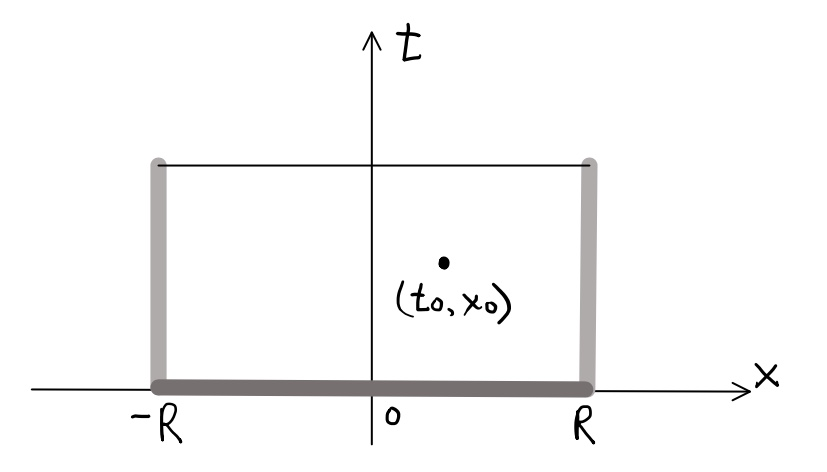
\includegraphics[scale=0.4]{cha11im1}
\end{center}

По принципу максимума на стакане $ u_\varepsilon \geq 0 $ в прямоугольнике. Значит $u_\varepsilon(t_0, x_0) \ge 0$, тогда $M - u(t_0, x_0) + \varepsilon \ge 0$, значит $u(t_0, x_0) \le M + \varepsilon$, т.е. $u_(t_0, x_0) \le M$ при $\varepsilon \longrightarrow 0$.

\end{Proof}

\begin{conseq}
Ограниченное решение задачи Коши единственно.
\end{conseq}

\begin{proof}
Допустим, что существуют два разные решения $u_1 \not = u_2$. Рассмотрим их разность $ z = u_1 - u_2 $. Запишем для $z$ задачу Коши:
$$\begin{cases}
	z_{t} = a^2 u_{xx}, \; t > 0, \; x \in \mathbb{R}\\
	z|_{t = 0} = 0 \\
    |z| \leq \tilde{C}, \; t \geq 0, \; x \in \mathbb{R}.
\end{cases}$$

По принципу максимума получаем $ z \equiv 0$, откуда $u_1 = u_2$.
\end{proof}


